\section{Architekturkonzept}
\label{sec:architekturkonzept}
    Das Framework stellt die Kern-Funktionalität zur Steuerung von implementierten Regeln und Prozessen innerhalb eines 
    Gebäudes, bspw. eines Büroraumes, dar. Mit dem Architekturkonzept wird der grundlegende Aufbau, sowie die Funktionalität des Systems erläutert. 
    Potentielle Erweiterungen und Adaptionen werden im Ausblick (\ref{chap:ausblick}) aufgegriffen.
    \\ 
    \linebreak
    Das System soll in drei Schichten aufgeteilt werden. Die oberste Schicht stell die Kommunikationsschicht dar, die mittlere Ebene 
    handelt um die Logik- und Prozessschicht und der unterste Block repräsentiert die Persistenzschicht. Im Rahmen der Arbeit wird 
    die dritte Schicht nicht detailliert beschrieben, da diese zu aktuellem Zeitpunkt keinen Nutzen generiert, bzw. für keine weitere Verarbeitung 
    genutzt wird. Die Ausprägung der Schicht ist dennoch ohne weiteres möglich und wird auch grob skizziert. Der Abbildung 
    (\ref{fig:schichtenarchitektur}) ist die Aufteilung der Schichtenarchitektur zu entnehmen. In der Darstellung unterscheidet sich die 
    Persistenzschicht von den anderen, um erkenntlich zu machen, dass diese in aktuellem Konzept keine konkrete Implementierung erfährt. 
    Durch die Darstellung in übergreifender Form wird deutlich, dass bereits auf dieser Ebene die Trennung der Zuständigkeiten, engl. 
    \textit{seperation of concerns}, greift. Durch die gezielte Abstraktion von Komponenten und Informationen kann die Komplexität 
    eines Systems gesteuert werden. Die Kommunikationsschicht ermöglicht die Anbindung von verschiedensten Kommunikationsprotokollen, die 
    dadurch schnell adaptiert werden können. Im Rahmen des Konzeptes wird ausschließlich Gebrauch des \acs{MQTT}-Protokolls gemacht. 
    Die Logikschicht nimmt alle eingehenden Events der Kommunikationsschicht entgegen, die jeweils eine Zustandsänderung erzwingen, 
    und durchläuft den Prozess des Frameworks, um auf die Zustandsänderung die passende Regel auszuführen. Die 
    Persistenzschicht ist für die Speicherung erzeugter Daten zuständig, bspw. wenn eine Transaktionshistorie von Zustandsänderungen 
    persistiert werden soll. Ebenso können Informationen gespeichert werden, die anderweitig zur Verfügung stünden. Das Vorantreiben der Speicherung 
    von Informationen kann durch den agilen Entwicklungsprozess außerhalb des Thesis-Rahmens erfolgen. 
    \begin{figure}[hbt!]
        \centering
        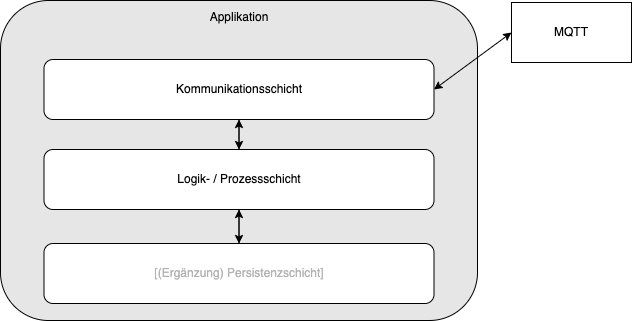
\includegraphics[width=14cm,height=10cm,keepaspectratio]{images/Schichtenarchitektur.png}
        \caption{Schichtenarchitektur}
        \label{fig:schichtenarchitektur}
    \end{figure}
    \\
    %\pagebreak
    Für die Konzeption von wartbarer und erweiterbarer Software, wird von den \textit{SOLID}-Prinzipien, sowie von nützlichen 
    und für das Framework verwendbaren Programmiermustern Gebrauch gemacht. Diese werden an geeigneter Stelle und auf den Nutzen bezogen erläutert.
    \\
    \linebreak
    Das \textit{SOLID} wurde von Robert C. Martin\footnote{Software Engineer, Lehrer und Autor Robert C. Martin. \url{https://en.wikipedia.org/wiki/Robert_C._Martin} Besucht am 10.07.2022} 
    geprägt und soll zum Design guter objektorientierter Software beitragen. Dadurch soll 
    ein Softwaresystem einer höheren Wartbarkeit unterliegen. Es setzt sich aus fünf Prinzipien zusammen, %\footnote{SOLID Prinzipien. \url{https://blog.cleancoder.com/uncle-bob/2020/10/18/Solid-Relevance.html} Besucht am 10.07.2022}, 
    die wie folgt definiert sind:
    \begin{itemize}
        \item S - Single-Responsibility-Prinzip: „Das Single-Responsibility-Prinzip (SRP; Eine-Verantwortlichkeit-Prinzip; ...) fordert, dass eine Klasse oder ein Modul einen und nur einen \textit{Grund zur Änderung} haben sollte.“ \cite{cleancode2009}
        \item O - Open-Closed-Prinzip: „Module sollten sowohl offen (für Erweiterungen) als auch verschlossen (für Modifikation) sein.“ \cite{ocpmeyer1988}
        \item L - Liskovsches Substitutionsprinzip: „... Sei q(x) eine beweisbare Eigenschaft von Objekten x des Typs T. Dann soll q(y) für Objektes des Typs S wahr sein, wobei S ein Untertyp von T ist.“ \cite{liskov2001behavioral} - Das (Ersetzungs-)Prinzip sagt somit aus, dass eine 
        Subklasse stets die Eigenschaften der Superklasse erfüllt und immer als Objekt der Superklasse anwendbar sein muss. Eine Subklasse darf dadurch erweitert werden, aber 
        keine grundlegende Änderung erfahren. 
        \item I - Interface-Segregation-Prinzip: „Clients sollen nicht dazu gezwungen werden, von Interfaces abzuhängen, die sie nicht verwenden.“ \cite{martin1996interface}
        \item D - Dependency-Inversion-Prinzip: „A. Module hoher Ebenen sollten nicht von Modulen niedriger Ebenen abhängen. Beide sollten von Abstraktionen abhängen. B. Abstraktionen sollten nicht von Details abhängen. Details sollten von Abstraktionen abhängen.“ \cite{martin2003agile}
    \end{itemize}
    Besonders das \textit{Single-Responsibility} und das \textit{Open-Closed}-Prinzip wurden bei der Konzeption berücksichtigt. 
    %Diese Prinzipien werden bei der Konzeption des Frameworks berücksichtigt. 
    Da es sich bei diesem System nicht um eine klassische 
    Webanwendung handelt und keine direkte Kommunikation unter anderem über \acs{REST} \acs{API}s stattfindet, wird ein allgemeines 
    Programmiermuster, wie bspw. das \ac{MVC}\footnote{Architekturmuster für Webapplikationen. \url{https://de.wikipedia.org/wiki/Model_View_Controller} Besucht am 10.07.2022} 
    oder das \ac{MVVM}\footnote{Software-Architekturmuster. \url{https://en.wikipedia.org/wiki/Model–view–viewmodel} Besucht am 10.02.2022 }, nicht 
    in Betracht gezogen. Verwendet werden allgemeine Architekturmuster und -prinzipien, die dazu beitragen die Software wartbar 
    zu gestalten, die Komplexität einzelner Funktionen zu reduzieren und die Lesbarkeit und Überschaubarkeit zu erhöhen. 
    
    \subsection{Aufbau des Frameworks}
        Nach Veranschaulichung der Schichten-Modellierung wird übergreifend der Komponenten Aufbau, sowie die dafür einzusetzenden Architekturmuster aufgegriffen. 
        \\
        Die Konzeptkomponenten (\ref{subsec:conceptcomps}) finden sich im umfassenden Architekturschaubild (siehe Abbildung \ref{fig:patternarchitektur}) wieder. 
        Die Regelstruktur 
        soll die Funktion einer Bedingungsprüfung und der darauffolgenden Aktion vorgeben, damit bestimmte Anhaltspunkte geschaffen sind, die das Framework überprüfen 
        und anwenden kann. Um zu gewährleisten, dass dem Anwender diese Methoden bei Implementierung einer spezifischen Regel zur Verfügung stehen, wird mittels dem 
        \textit{Template Method} Pattern \cite{gamma1995template} ein Leitfaden vorgegeben. Dieses gehört zu den Verhaltensmustern, engl. behavioral patterns. 
        Ziel des Schablonenmethoden-Entwurfsmusters ist die Delegation der konkreten Ausformung einzelner Methoden und Funktionen zu deren Unterklassen. Innerhalb der 
        abstrakten Klasse wird das Skelett des Objektes definiert. Die einzelnen Schritte können so in den darunter liegenden Klassen überschrieben oder ergänzt 
        werden, ohne dass die grundlegende Struktur der übergreifenden Klasse modifiziert werden muss. Die Unterklassen, die konkrete Definition einer Regel, sollen 
        unter Verwendung des \textit{Singleton} Patterns \cite{gamma1995singleton} realisiert werden. Das zu den Erzeugungsmustern 
        zugehörige Pattern dient zur 
        Sicherstellung, dass eine Klasse, in dem Fall die einzelne Regel, zur Laufzeit ausschließlich eine einzige Instanz erzeugt und diese global erreichbar ist. 
        Dadurch wird von jeder Regel immer nur ein Objekt erzeugt. 
        \\
        \linebreak
        Ähnlich zu dem Aufbau des Regelwerkes, sollen die Komponenten, die reale Gegenstände abbilden, ebenso Gebrauch des Schablonenmethoden-Entwurfsmusters machen. 
        Unterschied zu der Regel-Schablone ist lediglich die Funktion der Sperrung einer Komponenten für weitere Aufgaben. Diese soll bereits in der abstrakten Klasse 
        definiert sein. Konkrete Komponenten-Eigenschaften und Zustandsattribute können von dem Anwender selbst implementiert werden.
        \\
        \linebreak
        Die durch den Anwender implementierte Transformation, die unter anderem basierend auf einem eingehenden \acs{MQTT}-Topic das Zustandsobjekt verändert, soll %als Vorgabe 
        %stützend 
        das {Template Method} Pattern verwenden. Dadurch ist die Struktur der Transformation vorgegeben, die bei der Definition eines neuen Transformationsobjektes die zu 
        implementierenden Funktionen bereitstellt. %anhand dessen der Anwender neue Transformationsobjekte 
        %je nach Anwendungsfall erzeugen kann. 
        Innerhalb dieser Schablone sollen alle Attribute vorgegeben werden, die für die Transformation notwendig sind und von dem Softwareentwickler implementiert werden sollen. 
        \\
        \linebreak
        Damit zukünftig weitere Kommunikationsschnittstellen hinzugefügt werden können, soll für die Transformation zusätzlich das 
        \textit{Adapter} Pattern verwenden werden. Dadurch können Events aus unterschiedlichen Services und über mehrere Kommunikationswege 
        entgegengenommen werden, ohne dass die eigentliche Schnittstelle modifiziert werden muss. Das \textit{Adapter} Pattern gehört 
        zu den Strukturmustern und ist wie folgt definiert: 
        Die Konvertierung einer Schnittstelle einer Klasse in eine andere Schnittstelle, die vom Client erwartet wird. Dadurch ist die Zusammenarbeit von Klassen 
        gewährleistet, die sonst aufgrund der inkompatiblen Schnittstelle nicht zusammenarbeiten könnten. \cite{gamma1995adapter}
        \pagebreak
        \\
        Das Zustandsobjekt ist aus Anwendersicht als ein einfaches \ac{POJO}, ein ganz normales Java Objekt, zu implementieren. Das Framework soll sich um die korrekte Nutzung 
        des Objektes kümmern. 
        \\
        \linebreak
        Der übergreifende Aufbau unter Verwendung von Entwurfsmustern ist folgender Abbildung zu entnehmen:
        \begin{figure}[hbt!]
            \centering
            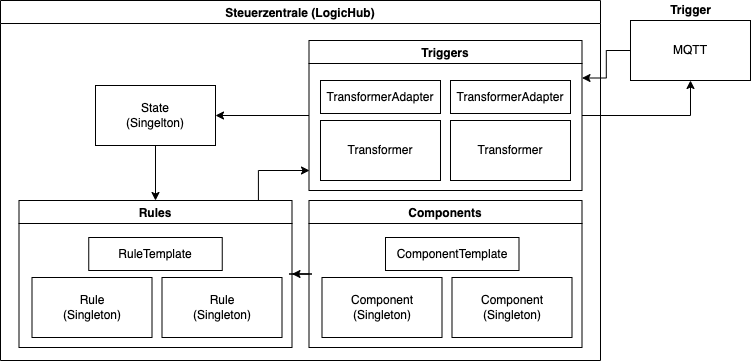
\includegraphics[width=14cm,height=10cm,keepaspectratio]{images/final_architecture_with_patterns.png}
            \caption{Architektur mit verwendeten Entwurfsmustern}
            \label{fig:patternarchitektur}
        \end{figure}
        \\
        Der soeben grob skizzierte Aufbau wird in den folgenden Abschnitten konkretisiert.

    \subsection{Kommunikationsschicht}
    Damit das Framework einer hohen Wartbarkeit und Erweiterbarkeit unterliegt, soll bereits in der Kommunikationsebene mithilfe 
    des genannten \textit{Adapter} Musters eine Abstraktionseben geschaffen werden. Diese erleichtert das Adaptieren 
    hinzukommender Kommunikationsschnittstellen. Im Rahmen der Arbeit und unter Verwendung des \acs{MQTT}-Kommunikationsprotokolls kann die 
    Konzeption der Kommunikationsschicht mithilfe des \textit{Adapter} Patterns dem Klassendiagramm der Abbildung (\ref{fig:patternarchitektur}) entnommen werden. 
    Der Client, in dem Fall der \acs{MQTT}-Topic-Subscriber, wird mit einem Transformationsadapter versehen. Hierbei werden die 
    Informationen, die über den Subscriber generiert werden, über eine Funktion an das Framework übergeben, sodass dieses mit den Eingangsinformationen arbeiten kann. 
    Wird eine weitere Kommunikationsschnittstelle hinzugefügt, so muss lediglich ein dafür vorgesehener \textit{Adapter} implementiert werden, der 
    alle für das Framework notwendigen Informationen übergibt. So bleibt die interne Arbeitsweise des Frameworks unverändert.
    \begin{figure}[hbt!]
        \centering
        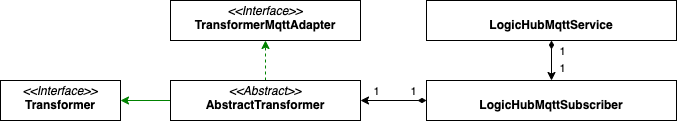
\includegraphics[width=14cm,height=10cm,keepaspectratio]{images/Kommunikationsschicht_final.png}
        \caption{Klassendiagramm der Kommunikationsschicht}
        \label{fig:patternkommunikation}
    \end{figure}
    \pagebreak
    \\
    Der interne Ablauf einer Nachrichtenkonsumierung kann dem Sequenzdiagramm in Abbildung (\ref{fig:kommunikationsequenz}) entnommen werden. Mit der Transformation 
    wird das eingehende \acs{MQTT}-Topic mit den vom Anwender definierten Topics überprüft. Gibt es dabei eine Übereinstimmung, so wird anhand des Topics die mitgelieferte 
    Nachricht konsumiert und dem jeweiligen Wert im Zustandsraum zugeordnet und dementsprechend verändert. Mit der Zustandsänderung wird die 
    Prozessschicht des Frameworks aufgerufen, die daraufhin die dem Framework bekannten Regeln überprüft und zutreffende startet. Der Durchlauf wird in dem Abschnitt (\ref{subsec:logikschicht}) 
    explizit dargestellt. 
    \begin{figure}[hbt!]
        \centering
        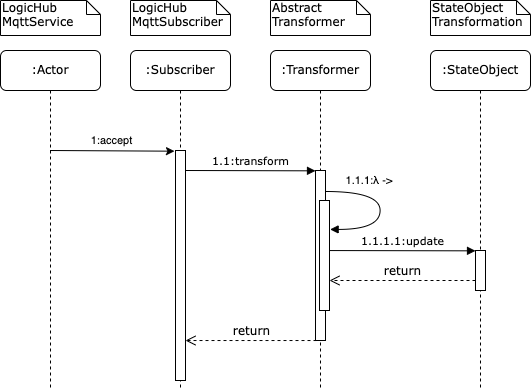
\includegraphics[width=14cm,height=10cm,keepaspectratio]{images/Kommunikationsschicht_Sequenz_Final.png}
        \caption{Sequenzdiagramm zur Kommunikationsschicht}
        \label{fig:kommunikationsequenz}
    \end{figure}
    % NOCHMALS DIE SCHICHTEN MIT:
    % KOMMUNIKATIONSSCHICHT UND AUFBAU -> \subsection{}?
    % LOGIKSCHICHT UND AUFBAU -> \subsection{}?
    \subsection{Logik- und Prozessschicht}
    \label{subsec:logikschicht}
    Die Logik- und Prozessschicht wird aktiv, wenn durch eine bestimmte Kommunikationsschnittstelle, im Rahmen der Arbeit ausschließlich durch \acs{MQTT} realisiert, ein eingehendes 
    Event, bzw. eine eingehende Nachricht konsumiert und daraufhin das Zustandsobjekt geändert wurde. Die in erster Linie dafür benötigten Objekte sind dem 
    Klassendiagramm (\ref{fig:patternlogik}) zu entnehmen. Die an zentraler Stelle stehende Klasse des \textit{LogicHubState} übernimmt die Koordination 
    der Zustandsänderung, sowie das nachträgliche Prüfen der Regelbedingungen, sowie das Ausführen des Regelprozesses. 
    \\
    Darin wird die Kopie des Zustandsobjektes inklusive der Änderung vorgenommen werden, damit in folgenden Prozessen die Repräsentation des Objektes nicht verfälscht wird. 
    Somit wird verhindert, dass eine durch Regeln erzeugte Zustandsänderung das eigentliche Objekt direkt manipuliert. Dies ist eine getroffene Maßnahme, da die Regelprozesse asynchron abgearbeitet werden 
    und so mehrere Zustandsänderungen erfolgen könnten. Zusätzlich ist der Kopiervorgang zu sperren, dass keine Inkonsistenz des Zustandes entsteht. 
    Dieser Vorgang wird in der Umsetzung (siehe Kapitel \ref{chap:umsetzung}) erläutert.
    \begin{figure}[hbt!]
        \centering
        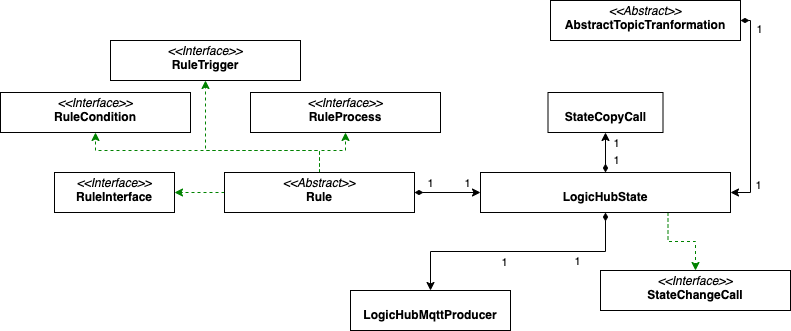
\includegraphics[width=14cm,height=10cm,keepaspectratio]{images/Logikschicht_final.png}
        \caption{Klassendiagramm zur Logik- und Prozessschicht}
        \label{fig:patternlogik}
    \end{figure}
    \\
    Der initiale Ablauf von der Erstellung einer Kopie, bis hin zur Prüfung der Regelbedingung, sowie das anschließende Durchführen gestaltet sich wie folgt: 
    \\
    \pagebreak
    \begin{figure}[hbt!]
        \centering
        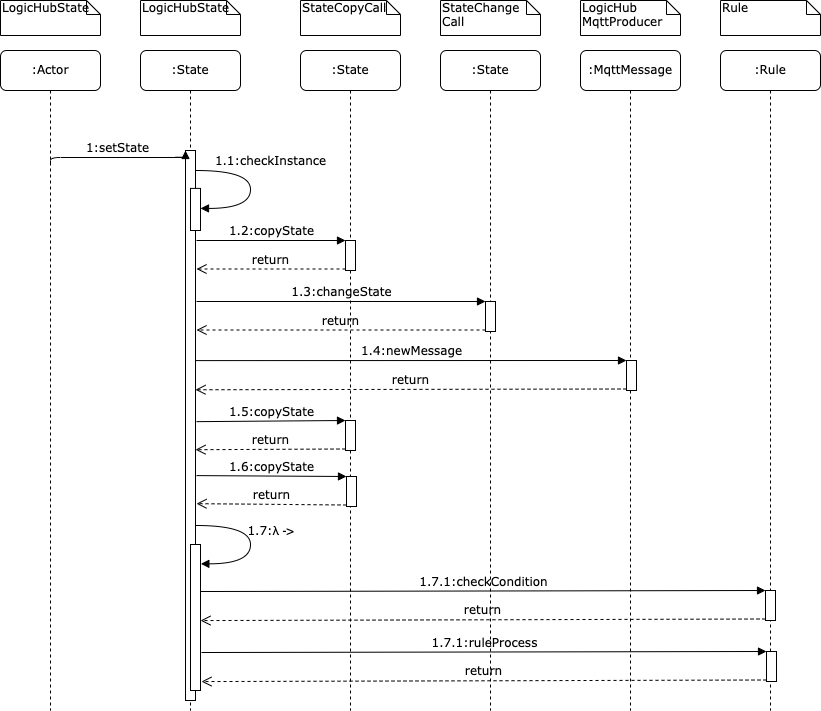
\includegraphics[width=14cm,height=14cm,keepaspectratio]{images/Logikschicht_Sequenz_final.png}
        \caption{Sequenzdiagramm zur Logikschicht}
        \label{fig:logiksequenz}
    \end{figure}
    \\
    \linebreak
    Dem Sequenzdiagramm ist ebenso die Transformation zu entnehmen, die erzielt wird, wenn durch eine Regel eine erneute Zustandsänderung stattfindet, die bspw. Befehle über \acs{MQTT} 
    veröffentlicht, um Komponenten steuern zu können. Auf die konkrete Umsetzung der soeben architektonisch beschriebenen Komponenten wird in folgendem Kapitel (siehe Umsetzung \ref{chap:umsetzung}) 
    eingegangen.
    \\
    Die Ausprägung der Persistenzsschicht wurde im Rahmen dieser Arbeit nicht weiter detailliert, da zu aktuellem Zeitpunkt 
    kein Bedarf an der Speicherung von Historien oder Zustandsänderungen besteht. Dennoch wird an dieser Stelle erwähnt, dass die Einbindung einer 
    Datenbank, sowie die Modellierung der Datenobjekte und deren Speicherung ohne weiteres möglich ist und dem keine Grenzen gesetzt sind.  
    %\subsection*{Persistenzschicht}
    % EVTL.: PERSISTENZSCHICHT UND POTENTIELLER AUFBAU -> \subsection{}?
    % Es wird alles abgebildet über einen Zustandsraum, der sich aus den Dingen (Gegenständen) und Zuständen der Anwendung ergibt.
    % Der Zustandsraum wird verändert, wenn eine Aktion durchgeführt wird, bzw. durch eine Trigger angestoßen. 
    % Bzw. speichert den aktuellen Zustand des Gegenstandes 
    % (lightBulb = true/false, personOnDoor = null/Mikka, booking = stringBooking, temiAktive = true/false, 
    % temiPosition = stringKoordinates)
    % Zustandsraum muss von dem Entwickler definiert werden. 
    % MQTT Broker über Home Assistant, bzw. losgelöster Broker
    % Anbindung von APIs auch Entwickler-Sache. Kann ich das vereinfachen, sodass die Integration einfacher wird?
    %\subsection{Überlegungen, Anstöße und Herausforderungen}
    % Regeln über Thread abbilden? Ja, Nein? - Nein, wieso? Da Durch die MQTT Message mehrere Regeln ausgeführt 
    %werden können. -> Lediglich den Zustand der Komponenten locken.
    % KEIN THREAD (wird schon abgebildet durch die Services und die Auslöser durch MQTT), Falls eine Komponente 
    %  doppelt beansprucht wird, ist der Zustand der Komponenten zu locken und ein 
    % Thread.sleep einzurichten. Abfrage, ob der Wert, bzw. die Komponente wieder freigegeben wurde. 
    % Zustandsraum -> Abbildung aller notwendigen Komponenten 
    % Bei Bearbeitung einer Regeln die Komponenten Locken, sodass nur die einzelne Komponenten (deren Zustand) gelockt ist 
    % und nicht der ganze Zustandsraum, somit können mehrere Komponenten und Aktionen ausführen zu können. 
    %Was brauche ich für Funktionen und Werte in einer Regel?
    % Ein Zustandsraum (Objekt) für alles oder ein Globales, welches die die Komponenten enthält? - Begründung für die Auswahl.
    %\subsection{Schnittstellen}
        % Kommunikation mit API's je nach Use Case und Gebrauch zur Datenabfrage
    %\subsection*{Datenbanken}
    %   Anbindungen an Datenbanken sind je nach hinzukommendem Anwendungsfall ohne weiteres möglich. Dies ist eine Konzeptvertiefung, die 
    %    im Rahmen dieser Arbeit nicht konkretisiert wird, da der Fokus auf der Kernfunktionalität, sowie auf dem 
        % Datenbanken je nach Use Case und Gebrauch zur Datenabfrage
    %\subsection{Parallelität}
    %HERAUSFORDERUNG MIT DEM QUEUEING ANTEASERN.
%\subsection{Softwarekonzept}
%\label{subsec:softwarekonzept}
\\
%\linebreak
Für die Generierung mehrerer konkurrierender Sichten, wurde unter Verwendung des \textit{4+1 Sichtenmodells} von Philippe Kruchten \cite{Kruchten1995}
bereits bei der Anforderungsanalyse (\ref{chap:anforderungsanalyse}) die Szenarien beschrieben. Die im Modell dargestellten Sichten wurden mit 
Klassen- und Sequenzdiagrammen %-, Aktivitäts- und Komponentendiagrammen 
im Konzept veranschaulicht. Nach Beendigung der Konzeption wird in folgendem Kapitel die Umsetzung des Konzeptes und die 
Implementierung des Prototypen vertieft. 
